\chapter{Data}\label{ch:style}
\usepackage{graphicx}
\usepackage[export]{adjustbox}
\section{TMK Dataset}
The TMK dataset was created by Goldsmith, Butcher, Benjamin, Sowmya, Muchlinski (2020) in  \emp{“Introducing The Targeted Mass Killing Dataset for the Study and Forecasting of Mass Atrocities”}
The TMK dataset was created to contribute to the study into various atrocities such as genoicide, politicide. The dataset records events from 1946-2019 and tracks a wide variety of socioeconomic factors. The scale of the TMK event is quantified via a pre-coded ordinal indicator that aggregates evidence of intent as well as number of deaths.

\begin{center}
 \begin{tabular}{||c c c||} 
 \hline
 Score & Intent & Total Deaths\\ [1ex] 
 \hline
 1 & NO Stated OR Organizational Intent & $25 \leq x \leq 999$ \\ [1ex] 
 \hline
 2 & NO Stated OR Organizational Intent &  $\geq 1000$  \\ [1ex] 
 \hline
 3 & Stated OR Organizational Intent & $25 \leq x \leq 999$ \\ [1ex]  
 \hline
  & TMK GENOCIDE/POLITICIDE THRESHOLD & \\
 \hline
 4 & Stated AND Organizational Intent  &  $\geq 1000$  \\ [1ex] 
 \hline
  5 & Stated AND Organizational Intent  & $25 \leq x \leq 999$  \\ [1ex] 
 \hline
  6 & Stated AND Organizational Intent  &  $\geq 1000$   \\ [1ex] 
 \hline
  7 & Stated AND Organizational Intent  &  $\geq 10,000$   \\ [1ex] 
 \hline
  8 & Stated AND Organizational Intent  &  $\geq 100,000$   \\ [1ex] 
 \hline
\end{tabular}
\end{center}

\section{Alternative Data Sources}
\subsection{Social Conflict Analysis Database}
\subsection{Uppsala Conflict Data Program}
\section{Political Instability Task Force}
web-pages~\cite{Noo05}.  The requirements below are for the written thesis
only.


\section{Data Issues}
\subsection{Class Imbalance}
\subsection{Missing Values}
Like most datasets in social science a lot of events have missing values
\subsubsection{Logical Imputations}
Logical imputation involves replacing missing values when the logic is obvious. For example, missing values can be logically imputated for TMK related because the dataset contains only TMK events

\subsubsection{Multivariate Imputation Chained Equations}
Multivariate Imputation via Chained Equations (MICE) 

\begin{center}
    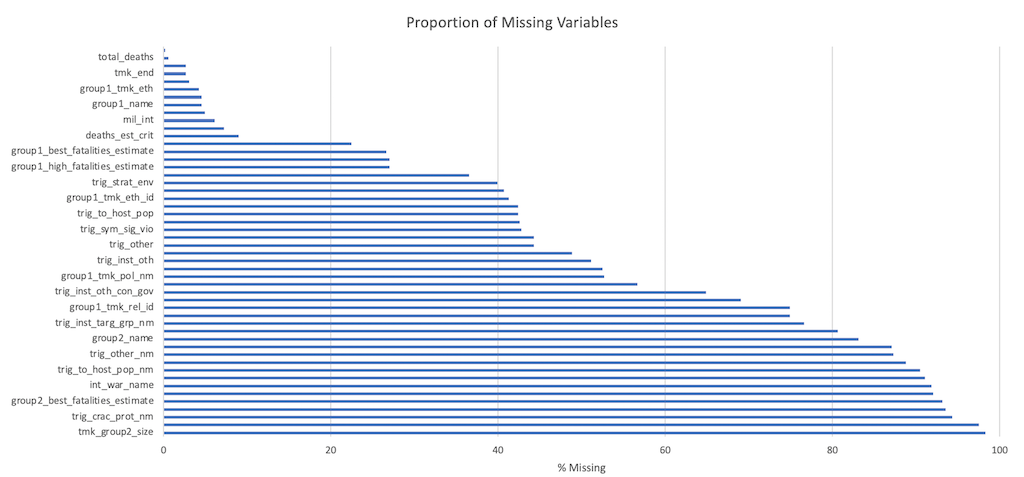
\includegraphics{Screen Shot 2021-04-17 at 15.01.40.png}
\end{center}



\subsection{Feature Explosion}
\section{Format}
The following format specifications must be adhered to for your thesis
(the \LaTeX\ template available from the school ensures this):
\begin{enumerate}
\item The thesis must be written on \emph{A4 size paper}.
\item The thesis must be typed or prepared using a \emph{word-processor}.
\begin{itemize}
\item For Undergraduate theses, you are encouraged to use both sides
  of the paper.
\item For Higher Degree Research theses, your submitted thesis must be
   printed single-sided.
\end{itemize}
\item \emph{Margins} on all sides must be no less than \unit[20]{mm} (before
binding).
\item \emph{1.5 line spacing} (about \unit[8]{mm} per line) must be used.
\item All sheets must be \emph{numbered}. The main body of the thesis must be
numbered consecutively from beginning to end.  Other sections must either
be included or have their own logical numbering system.
\item The \emph{title page} must contain the following information:
\begin{enumerate}
\item University and School names.
\item Title of Thesis/Project.
\item Name of Author and student ID.
\item The degree the thesis is submitted for.
\item Submission date (month and year).
\item Supervisor's name (for undergraduate theses).
\end{enumerate}
\item After the body of the thesis, the thesis \emph{must} contain a
  Bibliography or References list as appropriate.

Authors should confer with their supervisors and School about the
style of their bibliography, as this varies between disciplines.
\end{enumerate}

\section{Other physical appearance}
Other requirements to the physical appearance of your theses are:
\begin{enumerate}
\item \emph{Graphs, diagrams and photographs} should be inserted as close as
possible to their \emph{first reference} in the text. Rotated
graphs etc are to be arranged so as to be conveniently read, with the
bottom edge to the outside of the page.
\emph{Graphs and diagrams must be legible!}
\item \emph{Supplementary material (for example CFD animations)} may be submitted either online or via external drive, and must be referred to within the text. The text should make sense without the supplementary material available. 
\end{enumerate}

\section{Submission}

Finally, here are some requirements to the submission procedure. 

\begin{enumerate}
\item The \emph{author} of the thesis is \emph{responsible} for the preparation of the
thesis before the deadline, proofreading the
typescript and having corrections made as necessary.
\item For undergraduate theses, there is a \emph{page limit} of 50 pages for the main body of the thesis.
\end{enumerate}



\chapter{Content Requirements}\label{ch:content}

Students should consult the literature (e.g.~\cite{Sid99,StrWhi79,Coo64,GRS14})
and other resources for material on how to write a good
thesis.  The present document is only a very brief introduction as to what
is expected.

\nocite{NieLeh03,HasLehKwo05}

\section{Structure}
Most theses are structured very much like the present document.
The main part of the thesis can be structured in many different ways,
however, but must contain: a \emph{problem definition};
\emph{theory} and \emph{considerations} on how to solve the problem;
a description of the \emph{solution method} (dimensioning, construction,
etc.);
presentation of \emph{results} (measurements, simulations, etc.);
a \emph{discussion} of the results (validity, deviations, comparison
with previous solutions, etc.); and finally the \emph{conclusions}.

\section{Style of writing}

\begin{enumerate}

\item Audience:
The thesis must be addressed to engineers at the same level as the
student but without the special knowledge gained during the thesis work.
Such a third-person must be able to reconstruct the results on the basis
of the thesis alone.

\item
Every used concept/symbol/abbreviation which is not widely know must be \emph{defined}.
The wording should be \emph{short} and \emph{concise}.  
Readable(!) \emph{figures} and \emph{graphs} enhances comprehensibility.

\item Units.
\emph{SI units} must be used.
\end{enumerate}

\section{Documentation}

\begin{enumerate}
\item
The work must be well documented; i.e. enclosed must be the \emph{complete
schematics} of designed electronic circuits/test set-ups and/or a
\emph{program listing}, and/or etc.
Documentation of \emph{simulation results} and/or \emph{measurement
results} likewise.
\item References:
For every declaration/equation/method/etc., which is not widely known,
a \emph{reference to the literature} must be given (or a `proof' if it is
the authors own work).
In case material is copied verbatim, quotes must be used.
This is also the case when referring to partners
work in the case of a Group Thesis.

\item Plagiarism:
Failure to give proper references to the literature is \emph{plagiarism}.
Plagiarism is considered serious offence and severe penalties may apply.

\end{enumerate}

